\documentclass[11pt,a4paper]{article}
\usepackage[T1]{fontenc}
\usepackage{lmodern,microtype}
\usepackage[margin=28mm]{geometry}
\usepackage{amsmath,amssymb,amsthm,mathtools,mathrsfs}
\usepackage{enumitem,booktabs,xcolor}
\usepackage{tikz}
\usetikzlibrary{arrows.meta,positioning}
\usepackage[colorlinks=true,linkcolor=blue!45!black,citecolor=blue!45!black,urlcolor=blue!45!black]{hyperref}
\pdfinfoomitdate=1
\pdftrailerid{}
\pdfsuppressptexinfo=15
\emergencystretch=2em
\newcommand{\R}{\mathbb R}
\newcommand{\Q}{\mathbb Q}
\newcommand{\Z}{\mathbb Z}
\newcommand{\N}{\mathbb N}
\DeclareMathOperator{\Sym}{Sym}
\DeclareMathOperator{\tr}{tr}
\DeclareMathOperator{\supp}{supp}
\DeclareMathOperator{\rank}{rank}
\DeclareMathOperator{\diag}{diag}
\DeclareMathOperator{\Frac}{Frac}
\DeclareMathOperator{\adj}{adj}
\newtheorem{theorem}{Theorem}[section]
\newtheorem{proposition}[theorem]{Proposition}
\newtheorem{lemma}[theorem]{Lemma}
\newtheorem{corollary}[theorem]{Corollary}
\theoremstyle{definition}
\newtheorem{definition}[theorem]{Definition}
\theoremstyle{remark}
\newtheorem{remark}[theorem]{Remark}
\title{A classification of finite Euclidean Ramsey configurations}
\author{OpenAI}
\date{September 23, 2026}
\hypersetup{pdftitle={A classification of finite Euclidean Ramsey configurations},pdfauthor={OpenAI}}
\begin{document}
\maketitle
\begin{abstract}
We classify finite Euclidean Ramsey configurations by a necessary and
sufficient tensor condition over their coordinate fields. The Ramsey
property here concerns monochromatic congruent copies at the original
scale under arbitrary finite colorings. The criterion shows that every
nonempty subtransitive set and every nonempty set of at most five points
on a circle is Ramsey. In particular, some Ramsey cyclic quadrilaterals
are not subtransitive, disproving the necessity direction of the
Leader--Russell--Walters conjectured characterization.
\end{abstract}
\tableofcontents
\section{The classification problem}

A finite nonempty set $A$ in a Euclidean space is \emph{Ramsey} if, for
every integer $r\ge2$, there is an integer $D\ge1$ such that every map
$c:\R^D\to\{1,\ldots,r\}$ is constant on a congruent copy of $A$.
Congruence means preservation of every pairwise distance, at the original
scale. The coloring is an arbitrary function. In particular, no
measurability or other regularity is assumed.

Erd\H{o}s, Graham, Montgomery, Rothschild, Spencer and Straus introduced
Euclidean Ramsey theory and proved that every finite Ramsey set is
spherical~\cite[Theorem~13]{egm-rss}. Graham later conjectured that
sphericity is also sufficient~\cite{graham-survey}. Major positive
results established the Ramsey property for nondegenerate triangles
and then all nondegenerate simplices, by Frankl and
R\"odl~\cite{frankl-rodl-triangles,frankl-rodl-simplices}; finite sets
with a soluble transitive isometry group and cyclic trapezoids, by
K\v{r}\'i\v{z}~\cite{kriz-permutation,kriz-trapezoids}; and vertex sets
of regular polytopes, by Cantwell~\cite{cantwell-polytopes}.

Leader, Russell and Walters proposed a different characterization:
a finite set is Ramsey exactly when it embeds in a finite transitive
Euclidean set~\cite[Conjecture~A]{lrw-transitive}. Transitivity means
that the isometries of the finite set act transitively on its points.
An isometric subset of such a set is called \emph{subtransitive}.
Their group-theoretic and Hales--Jewett formulations led to the
Block Sets Conjecture; subsequent work studies the possible block
sizes~\cite{ilw-blocks}. The link with soluble symmetry has also
expanded: Karamanlis embedded every simplex in a finite product of
regular polygons~\cite{karamanlis-tori}, and Behague constructed
soluble transitive extensions for many known Ramsey classes and
further permutation configurations~\cite{behague-subsoluble}.
Ivan, Leader and Walters developed generalized-prism constructions,
with Ramsey conclusions under a soluble symmetry
hypothesis~\cite{ilw-prisms}. Moore and, independently, Mirabi proved
that adjoining a point outside the affine span of a Ramsey set
preserves the Ramsey property~\cite{moore-pyramid,mirabi-extensions}.
The affine-span restriction leaves the case of arbitrary coplanar
circle points beyond this extension theorem.

P\'alv\"olgyi has recently given a seven-point circle configuration
that is not Ramsey, disproving the spherical
conjecture~\cite[Theorem~1]{palvolgyi-heptagon}.
The appendix to that version also states that generic seven-point circle
configurations are not Ramsey. Its author's note announces a proof that
all finite transitive sets are Ramsey and says that its exposition is
still being prepared.\footnote{P\'alv\"olgyi attributes the writing, proofs, and
ideas in that manuscript to ChatGPT. He labels the additional appendix
claims as unchecked by him.}
Our main theorem gives a necessary and sufficient algebraic condition
for an arbitrary finite Euclidean configuration.

\subsection{The exact tensor criterion}

The problem is to characterize these finite sets up to congruence.
A singleton is Ramsey. For any other set, let $d\ge1$ be its affine
dimension, and choose a congruent representative
$A=\{a_1,\ldots,a_s\}\subset\R^d$ whose affine span is $\R^d$.
The points are distinct and $s\ge2$. Define
\[
 p_i=\begin{pmatrix}1\\a_i\end{pmatrix},\qquad
 F=\Q\bigl((a_i)_\alpha:1\le i\le s,\ 1\le\alpha\le d\bigr),
 \qquad B=F\otimes_{\Q}F.
\]
The commutative ring $B$ has a multiplication homomorphism
\[
 m_F:B\longrightarrow F,\qquad m_F(x\otimes y)=xy.
\]
An equality in $B$ is stronger than the equality obtained by applying
$m_F$; this map need not be injective. Index the entries of $p_i$ and
the rows and columns of a $(d+1)$-by-$(d+1)$ matrix by $0,1,\ldots,d$.
Thus index $0$ is the constant coordinate.

\begin{theorem}[Classification]\label{thm:classification}
Let $A=\{a_1,\ldots,a_s\}\subset\R^d$ be a finite set of at least two
points with affine span $\R^d$, and define $p_i,F,B,m_F$ as above.
Then $A$ is Ramsey if and only if there is a matrix
$P\in\operatorname{Mat}_{d+1}(B)$ such that
\begin{align}
 (p_i\otimes1)^T P(1\otimes p_i)&=0
       &&(1\le i\le s),\label{eq:field-evaluations}\\
 m_F(P_{\alpha\beta})&=\delta_{\alpha\beta}
       &&(1\le\alpha,\beta\le d).\label{eq:field-spatial}
\end{align}
Here the entries of $p_i\otimes1$ and $1\otimes p_i$ are formed
componentwise. There are no separate conditions on the multiplied
constant row or constant column of $P$.
\end{theorem}

The condition is independent of the chosen congruent representative
in its affine dimension; we also prove this directly through its tensor
formulation. It uses exact relations in the coordinate field. It is
not a procedure for recovering those relations from numerical
approximations to arbitrary real coordinates.

\subsection{Geometric consequences}

Applying $m_F$ to the evaluation equations gives an ordinary sphere
equation
\[
 \|a_i\|^2+\ell\cdot a_i+c=0\qquad(1\le i\le s)
\]
for some $\ell\in F^d$ and $c\in F$. The tensor condition requires the
evaluation identities to hold before multiplication. This is the
distinction between sphericity and the Ramsey property that the
classification detects.

Every subtransitive set satisfies the tensor condition. Another
sufficient condition is that evaluation at the points of a spherical
set gives independent functionals on the space of quadratic
polynomials. It applies to every nonempty set of at most five points
on a circle, and hence to every cyclic quadrilateral. In
Corollary~\ref{cons:kites}, we combine this result with the
non-subtransitive cyclic kites of Leader, Russell and
Walters~\cite[Corollary~2]{lrw-kites}. Those kites are Ramsey, disproving
the necessity direction of their proposed characterization and their
non-Ramseyness conjecture for the same family~\cite[Conjecture~3]{lrw-kites}.

For negative examples, nine points obtained from algebraically
independent real parameters in a rational parametrization of a circle
fail the tensor condition. P\'alv\"olgyi's generic seven-point
claim~\cite[Theorem~A.3]{palvolgyi-heptagon} already implies this
non-Ramseyness conclusion; our determinant calculation illustrates
how to apply the classification directly. We also give a tensor
obstruction for a twelve-point configuration consisting of three
rotated coordinate squares, using the same type of weighted derivation
moments as his heptagon construction. These consequences are proved
after the classification and require no further Ramsey construction.

\subsection{How the algebra forces a monochromatic copy}

The proof begins by replacing the coordinate-field matrix with a
finite rational combination of tensors of affine functions on
$\R^d$. Its evaluations at all points of $A$ vanish as rational
tensors, while its gradient Gram matrix is $I_d$.
If no such tensor exists, algebraic separation produces a finite
coloring that avoids $A$ in every dimension. This proves necessity.

For sufficiency, the difficulty is to convert the tensor cancellations
into a congruent copy at scale one: arbitrary colorings provide no
continuity with which to absorb approximation errors. The proof has
three stages.

First, the tensor determines signed rational multiplicities for a
finite list of affine functions. At every point of $A$, the positive
and negative multiplicities cancel separately at each evaluation
value. A Gaussian construction, followed by discretization and rational
approximation within a fixed convolution image, makes the negative
gradient second moment small while retaining these cancellations
exactly. The positive and negative multiplicities then give two lists
of affine functions. Evaluating the lists at $a_i$ gives vectors
$f_i,g_i$ with
\[
 \|f_i-f_j\|^2=\|a_i-a_j\|^2,\qquad
 \|g_i-g_j\|^2=q\|a_i-a_j\|^2,
\]
where $q>0$ can be arbitrarily small, and each $g_i$ is a coordinate
permutation of $f_i$. Both the distances and the matching coordinate
multisets are exact.

Second, we associate a free-group generator to each real sequence with
finite support. A \emph{path} is an ordered product of $s$-tuples:
each factor either records an ordered scaled copy of $A$ or has the
same group element in every position. Its \emph{endpoint} is the
coordinatewise product, and its \emph{weight} is the sum of the squared
copy scales. We prove that equal endpoints with arbitrarily small
weight ratios force the Ramsey property. The obstacle, familiar from
the group and word methods of Leader, Russell and
Walters~\cite[Sections~2--3]{lrw-transitive}, is the initially unknown
number $t$ of variable positions in a Hales--Jewett line. After fixing
the Hales--Jewett word length $n$, we prepare one endpoint at weights
$1,1/2,\ldots,1/n$ before coloring the words.
An ultrafilter construction then realizes the products by finite
strings, keeping common factors identical. The $t$ variable positions
give squared-distance multiplier $t(1/t)=1$. Compactness supplies a
finite ambient dimension for each number of colors.

Third, the permutation pairs from the first stage must be made to have
equal path endpoints. Permutation averaging puts the discrepancies
between their group entries in a subgroup whose elements can be
corrected by appending paths of unit-scale copies. Further averaging
makes the total correction weight small relative to the larger
original weight. Appending these corrections produces the equal
endpoints and arbitrarily small weight ratios required in the second
stage.

Sections~\ref{sec:tensors}--\ref{pairs:section} establish the algebraic
formulation, necessity, and the exact pair construction.
Section~\ref{paths:section} states and proves the group-endpoint criterion
that suffices for Ramsey forcing. Section~\ref{sec:groups} constructs
the required endpoints and completes the proof of
Theorem~\ref{thm:classification}. Section~\ref{cons:section}
derives the geometric examples. All arguments take place in ZFC.

\section{Rational tensors and the coloring obstruction}\label{sec:tensors}

We first express the matrix condition of Theorem~\ref{thm:classification}
as a condition on affine functions.  This formulation makes the obstruction
to arbitrary colorings explicit and supplies the input for the construction
in the next section.  Throughout, $s\geq2$, $d\geq1$, and
$A=\{a_1,\ldots,a_s\}$ affinely spans $\R^d$; the field $F$, ring $B$,
columns $p_i$, and multiplication map $m_F$ are as in the theorem.

Put $W=\R\times\R^d$, regarded as a vector space over $\Q$.
An element $w=(v,u)$ specifies the affine function $a\mapsto v+a\cdot u$.
For each label define the $\Q$-linear evaluation map
\[
 e_i:W\longrightarrow\R,\qquad e_i(v,u)=v+a_i\cdot u.
\]
Let $\mathcal T(W)$ be the subspace of $W\otimes_{\Q}W$ fixed by the
flip $w\otimes w'\mapsto w'\otimes w$.  Thus our symmetric tensors are
flip-invariant tensors.  The map
\[
 (v,u)\otimes(v',u')\longmapsto u(u')^{\mathsf T}
\]
is $\Q$-linear on the tensor product and restricts to a map
$G:\mathcal T(W)\to\Sym_d(\R)$, where $\Sym_d(\R)$ denotes the real
symmetric matrices.  In particular, $G(w\otimes w)=uu^{\mathsf T}$.
The tensor condition is the existence of $T\in\mathcal T(W)$ such that
\begin{equation}\label{alg:tensor}
 (e_i\otimes e_i)(T)=0\quad(1\leq i\leq s),
 \qquad G(T)=I_d.
\end{equation}
The first identities hold in $\R\otimes_{\Q}\R$.
They are stronger than their images under real multiplication.

\begin{proposition}\label{alg:equivalence}
The matrix condition in Theorem~\ref{thm:classification} is equivalent
to~\eqref{alg:tensor}.
\end{proposition}

\begin{proof}
Write $\mathscr B=\R\otimes_{\Q}\R$, let
$\tau(x\otimes y)=y\otimes x$, and let
$m_{\R}:\mathscr B\to\R$ be multiplication.
The coordinate decomposition of $W$ identifies $W\otimes_{\Q}W$ with
arrays $Q=(Q_{\alpha\beta})_{0\leq\alpha,\beta\leq d}$ over $\mathscr B$.
Under this identification, evaluation is
\[
 E_i(Q)=\sum_{\alpha,\beta=0}^d
 (p_{i,\alpha}\otimes1)Q_{\alpha\beta}
 (1\otimes p_{i,\beta}),
\]
and the gradient matrix is the spatial block
$(m_{\R}(Q_{\alpha\beta}))_{1\leq\alpha,\beta\leq d}$.
Tensor flip becomes
\[
 Q^*_{\alpha\beta}=\tau(Q_{\beta\alpha}).
\]
Directly from the evaluation formula,
$E_i(Q^*)=\tau(E_i(Q))$, and multiplication of $Q^*$ transposes the
multiplied array.  Consequently $\tfrac12(Q+Q^*)$ preserves every zero
evaluation and any multiplied spatial block equal to $I_d$.
This proves the implication from a matrix over $B$ to a symmetric tensor,
using the natural inclusion $B\subset\mathscr B$.

For the converse, we show that extending the coefficient ring from $B$
to $\mathscr B$ introduces no new solutions.  Choose an $F$-basis
$(r_\lambda)_{\lambda\in\Lambda}$ of $\R$.  Distributing tensor products
over direct sums gives the free $B$-module decomposition
\begin{equation}\label{alg:free-expansion}
 \mathscr B=
 \bigoplus_{\lambda,\mu\in\Lambda}
 B(r_\lambda\otimes r_\mu).
\end{equation}
Here a coefficient $x\otimes y\in B$ in the indicated summand represents
$(xr_\lambda)\otimes(yr_\mu)$.
If an array $Q$ over $\mathscr B$ solves the evaluation equations and has
multiplied spatial block $I_d$, its entries have a common finite expansion
\[
 Q=\sum_{(\lambda,\mu)\in J}
 (r_\lambda\otimes r_\mu)P^{\lambda\mu},
 \qquad P^{\lambda\mu}\in\operatorname{Mat}_{d+1}(B).
\]
All coefficients in the maps $E_i$ belong to $B$.
Thus~\eqref{alg:free-expansion} implies
$E_i(P^{\lambda\mu})=0$ for each pair and each label.
Let $C^{\lambda\mu}\in\operatorname{Mat}_d(F)$ be the multiplied spatial
block of $P^{\lambda\mu}$.  Applying multiplication to the expansion gives
\[
 I_d=\sum_{(\lambda,\mu)\in J}
 r_\lambda r_\mu C^{\lambda\mu}.
\]
This finite linear system has coefficients and right-hand side in $F$.
Since it is consistent over $\R$, row reduction over $F$ shows that it
is consistent over $F$.  Choose $c_{\lambda\mu}\in F$ with
$I_d=\sum c_{\lambda\mu}C^{\lambda\mu}$.  Then
\[
 P=\sum_{(\lambda,\mu)\in J}
 (c_{\lambda\mu}\otimes1)P^{\lambda\mu}
\]
is a solution over $B$.  The individual matrices $C^{\lambda\mu}$ need
not be symmetric; the descent took place in the full space
$\operatorname{Mat}_d(F)$.  If a symmetric tensor is wanted after descent,
the symmetrization already proved applies to $P$.
\end{proof}

\begin{remark}\label{alg:noetherian}
The finite coordinate presentation explains the algebraic nature of the
criterion.  Let $F_0=\Q[(a_i)_j]$, the subring of $\R$ generated by all
coordinates.  It is a finitely generated domain and $F=\operatorname{Frac}(F_0)$.
The ring $B$ is the localization of $F\otimes_{\Q}F_0$ at the elements
$1\otimes f$ for $0\ne f\in F_0$.  The latter ring is a finitely generated
$F$-algebra, so $B$ is Noetherian.
The kernel of the finite evaluation system therefore has finitely many
$B$-module generators.  Its multiplied spatial image is the $F$-span of
their multiplied spatial blocks, because every scalar $c\in F$ lifts to
$c\otimes1$.  This description uses exact coordinate-field relations;
it makes no claim to recover those relations from numerical real inputs.
\end{remark}

\begin{remark}\label{alg:congruence}
The tensor condition is directly invariant under congruence.
If $a_i'=Qa_i+t$ with $Q\in O(d)$, the invertible $\Q$-linear map
\[
 H:W\longrightarrow W,\qquad
 H(v,u)=(v-t\cdot Qu,Qu)
\]
satisfies $e_i'\circ H=e_i$ and
$G((H\otimes H)T)=QG(T)Q^{\mathsf T}$.
It therefore carries certificates for $A$ to certificates for $A'$;
the inverse congruence gives the converse.  Reordering labels merely
reorders the equations.  Any two congruent representatives in their
affine dimension are related by such a map, so
Proposition~\ref{alg:equivalence} also proves representative independence
for the matrix criterion, even when their coordinate fields differ.
\end{remark}

We next prove the necessary direction of the classification.
Failure of~\eqref{alg:tensor} gives an algebraic functional, and its values
provide a fixed finite coloring that works in every ambient dimension.
The invariant-and-coloring strategy goes back to Erd\H{o}s et al.
\cite[Theorem~13 and Lemma~15]{egm-rss}; here rational tensor separation
supplies the invariant, and the modular coloring is proved directly.
Their real-variable coloring lemma extends Rado's work on partition
regularity \cite{rado-note}.

\begin{proposition}\label{alg:necessity}
If~\eqref{alg:tensor} has no solution, then there is an integer $r_0\geq2$
such that every $\R^D$ admits an $r_0$-coloring with no monochromatic
congruent copy of $A$.  In particular, every Euclidean Ramsey set
satisfies the matrix condition of Theorem~\ref{thm:classification}.
\end{proposition}

\begin{proof}
Regard
\[
 \mathcal Y=(\R\otimes_{\Q}\R)^s\oplus\Sym_d(\R)
\]
as a $\Q$-vector space and define the $\Q$-linear map
\[
 \Phi:\mathcal T(W)\longrightarrow\mathcal Y,
 \qquad
 \Phi(T)=\bigl((e_i\otimes e_i)(T)\bigr)_{i=1}^s\oplus G(T).
\]
By assumption $y_0=(0,\ldots,0,I_d)$ is outside its image.
In the quotient vector space $\mathcal Y/\operatorname{im}\Phi$, extend
the nonzero class of $y_0$ to a basis over $\Q$.
Sending that basis element to $1$ and the others to $0$ gives a
$\Q$-linear functional $\ell:\mathcal Y\to\R$ such that
\[
 \ell\circ\Phi=0,\qquad \ell(y_0)=1.
\]
Write its components as $\ell_i:\R\otimes_{\Q}\R\to\R$ and
$L:\Sym_d(\R)\to\R$, and put $h_i(x)=\ell_i(x\otimes x)$.
Applying $\ell$ to $\Phi(w\otimes w)$ gives
\begin{equation}\label{alg:separated}
 \sum_{i=1}^s h_i(v+a_i\cdot u)+L(uu^{\mathsf T})=0,
 \qquad L(I_d)=1.
\end{equation}
Taking $u=0$ shows that
\begin{equation}\label{alg:constant-cancellation}
 \sum_{i=1}^s h_i(x)=0\qquad(x\in\R).
\end{equation}
These are purely algebraic functionals; no continuity or measurability is
asserted or needed.

Fix $D$ and define
$H_i(z)=\sum_{j=1}^D h_i(z_j)$ for $z\in\R^D$.
We claim that every ordered congruent copy $(b_1,\ldots,b_s)$ satisfies
\begin{equation}\label{alg:copy-obstruction}
 \sum_{i=1}^s H_i(b_i)=-1.
\end{equation}
Indeed, equality of the pairwise distances gives equality of the Gram
matrices of $(a_i-a_1)_i$ and $(b_i-b_1)_i$ by polarization.
Thus sending each $a_i-a_1$ to $b_i-b_1$ defines an inner-product-preserving
linear map on their span: any relation among the first differences has
squared norm zero for the corresponding combination of the second.
Since $A$ affinely spans $\R^d$, there are a linear isometry
$Q:\R^d\to\R^D$ and $t\in\R^D$ such that $b_i=t+Qa_i$.
Writing $u_j^{\mathsf T}$ for the $j$th row of $Q$, we have
\[
 (b_i)_j=e_i(t_j,u_j),\qquad
 \sum_{j=1}^D u_ju_j^{\mathsf T}=Q^{\mathsf T}Q=I_d.
\]
Sum~\eqref{alg:separated} over $j$.
The finite additivity of $L$ proves~\eqref{alg:copy-obstruction}.
Also~\eqref{alg:constant-cancellation} gives
$\sum_iH_i(z)=0$ at every single point $z$.

Choose $K=2s+1$ and partition $[0,2)$ into $K$ half-open intervals
of equal length $2/K<1/s$.  Color a point $z$ by the $s$-tuple of interval
labels of the representatives of $H_i(z)$ modulo $2$.
This uses at most $r_0=K^s$ colors, independently of $D$.
If $b_1,\ldots,b_s$ were monochromatic, there would be integers $n_i$
and real numbers $\varepsilon_i$, with $|\varepsilon_i|<2/K$, such that
\[
 H_i(b_i)-H_i(b_1)=2n_i+\varepsilon_i.
\]
Summation yields
\[
 -1=2\sum_i n_i+\sum_i\varepsilon_i,
 \qquad \left|\sum_i\varepsilon_i\right|<1.
\]
The first identity makes the error sum an odd integer, contradicting the
second.  This coloring avoids $A$ in every dimension and completes the
proof.
\end{proof}

The remaining direction begins with a tensor satisfying
\eqref{alg:tensor}.  Its evaluations vanish before multiplication, and
that exact cancellation will produce equal coordinate histograms for
two embeddings at different scales.

\section{A finite lattice identity}\label{stencil:section}

Assume that the tensor condition holds. We begin the sufficiency proof by
turning its rational tensor equalities into exact cancellation identities
for finitely many affine functions. These identities will let us construct
two copies of the configuration at different scales whose corresponding
points have the same coordinates in different orders.

Recall that $W=\R\times\R^d$ is viewed over $\Q$, and that
$e_i(v,u)=v+a_i\cdot u$. Let $T\in W\otimes_{\Q}W$ be symmetric, with
\[
 (e_i\otimes e_i)T=0\quad(1\leq i\leq s),
 \qquad G(T)=I_d.
\]
A tensor uses only finitely many vectors. Choose a basis
$w_1,\ldots,w_k$ over $\Q$ for a finite-dimensional subspace containing
its factors, and write
\[
 T=\sum_{a,b=1}^k C_{ab}w_a\otimes w_b,
 \qquad C\in\operatorname{Mat}_k(\Q),\quad C=C^{\mathsf T}.
\]
For $\lambda\in\Q^k$, put
\[
 w(\lambda)=\sum_{j=1}^k\lambda_jw_j.
\]
Write $w_j=(v_j,u_j)$ and let $U=(u_1\ \cdots\ u_k)$ be the real
$d\times k$ matrix whose columns are their gradients. The gradient
identity for $T$ is
\begin{equation}\label{stencil:gram}
 UCU^{\mathsf T}=I_d.
\end{equation}

Set $\Gamma=\Z^k$ and define the evaluation lattices
\[
 \Lambda_i=\{\lambda\in\Gamma:e_i(w(\lambda))=0\},
 \qquad V_i=\operatorname{span}_{\Q}\Lambda_i.
\]
Clearing denominators shows that $V_i$ is the kernel of the rational
linear map $\lambda\mapsto e_i(w(\lambda))$ on $\Q^k$.
Thus $\Q^k/V_i$ embeds into $\R$ over $\Q$. Tensoring this injection
with itself remains injective, so the tensor represented by $C$ has zero
image in $(\Q^k/V_i)\otimes_{\Q}(\Q^k/V_i)$.

The next lemma converts these tensor equalities into a finitely
supported rational function on $\Gamma$. Vanishing of its sums on each
coset will record exact cancellation among equal evaluations.

\begin{lemma}[Finite lattice identity]\label{stencil:finite}
Let $k,s\geq1$, let $\Lambda_1,\ldots,\Lambda_s$ be subgroups of
$\Gamma=\Z^k$, and put $V_i=\operatorname{span}_{\Q}\Lambda_i$.
Let $C\in\operatorname{Mat}_k(\Q)$ be symmetric. Suppose that the
image of
$\sum_{a,b}C_{ab}\varepsilon_a\otimes\varepsilon_b$
in $(\Q^k/V_i)\otimes_{\Q}(\Q^k/V_i)$ is zero for every $i$,
where $\varepsilon_1,\ldots,\varepsilon_k$ is the standard basis of
$\Q^k$. There is a finitely supported function $\nu:\Gamma\to\Q$
such that
\begin{equation}\label{stencil:cosets}
 \sum_{\gamma\in q}\nu(\gamma)=0
 \qquad(q\in\Gamma/\Lambda_i,\ 1\leq i\leq s)
\end{equation}
and
\begin{equation}\label{stencil:moments}
 \sum_\gamma\nu(\gamma)=0,\qquad
 \sum_\gamma\nu(\gamma)\gamma=0,\qquad
 \sum_\gamma\nu(\gamma)\gamma\gamma^{\mathsf T}=C.
\end{equation}
\end{lemma}

\begin{proof}
The Laurent polynomial ring
\[
 R=\Q[X_1^{\pm1},\ldots,X_k^{\pm1}]
\]
is the group algebra of $\Gamma$, with $X^\gamma=\prod_jX_j^{\gamma_j}$.
The quotient map $\Gamma\to\Gamma/\Lambda_i$ induces a ring
homomorphism whose kernel is
\[
 J_i=(X^h-1:h\in\Lambda_i).
\]
Indeed, its kernel consists of Laurent polynomials with zero coefficient
sum on each coset. Within a coset, choose a representative $\gamma_0$
from the finite support; a zero-sum polynomial on that coset is a sum of
terms $c_\gamma(X^\gamma-X^{\gamma_0})$, each in $J_i$.

We will find a Laurent polynomial in every $J_i$ with prescribed
terms through degree two near $X=(1,\ldots,1)$.
To use the tensor hypothesis, we pass to formal logarithmic coordinates,
in which the generators $X^h-1$ become linear forms multiplied by units.
Put $\mathfrak m=(X_1-1,\ldots,X_k-1)$ and complete $R$ with respect
to $\mathfrak m$. With $Z_j=X_j-1$, its completion is
$\widehat R=\Q[[Z_1,\ldots,Z_k]]$: the factors $1+Z_j$ are already
invertible modulo each power of $(Z_1,\ldots,Z_k)$.
The formal changes of variables
\[
 Y_j=\log(1+Z_j),\qquad Z_j=\exp(Y_j)-1
\]
identify this ring with $\Q[[Y_1,\ldots,Y_k]]$ and identify
$\mathfrak m\widehat R$ with $(Y_1,\ldots,Y_k)$.
For each $h\in\Gamma$,
\[
 X^h-1=\exp(h\cdot Y)-1
       =(h\cdot Y)\sum_{n\geq0}\frac{(h\cdot Y)^n}{(n+1)!}.
\]
The final factor is a unit. Hence
\begin{equation}\label{stencil:linear-ideals}
 J_i\widehat R=(h\cdot Y:h\in\Lambda_i)\widehat R.
\end{equation}

Consider the quadratic polynomial
\[
 Q_2(Y)=\tfrac12Y^{\mathsf T}CY.
\]
Identify $\Q[Y_1,\ldots,Y_k]$ with the symmetric algebra of $\Q^k$
by sending $\varepsilon_j$ to $Y_j$. The map to the symmetric algebra
of $\Q^k/V_i$ has kernel generated by $V_i$ in degree one. This follows, for example,
by extending a basis of $V_i$ to a basis of $\Q^k$.
The tensor hypothesis therefore puts $Q_2$ in the ideal generated by
the linear forms $h\cdot Y$, $h\in\Lambda_i$. By
\eqref{stencil:linear-ideals}, $Q_2\in J_i\widehat R$ for every $i$.

The ring $R$ is Noetherian, being a localization of a polynomial ring
over $\Q$. Its $\mathfrak m$-adic completion is therefore flat over
$R$ \cite[Lemma~10.97.2, Tag~00MB]{stacks-completion}.
If $I=\bigcap_{i=1}^sJ_i$, the injection
\[
 R/I\longrightarrow\bigoplus_{i=1}^sR/J_i
\]
remains injective after tensoring with $\widehat R$. Consequently
\[
 I\widehat R=\bigcap_{i=1}^sJ_i\widehat R,
\]
and $Q_2\in I\widehat R$.

We now recover a finite Laurent polynomial while retaining exact
membership in $I$. Write
\[
 Q_2=\sum_{a=1}^N f_a\alpha_a,
 \qquad f_a\in I,\quad\alpha_a\in\widehat R,
\]
as a finite sum. For each $a$, truncate the formal $Z$-expansion of
$\alpha_a$ through degree two to obtain $b_a\in R$ with
$b_a-\alpha_a\in\mathfrak m^3\widehat R$.
Then $f=\sum_af_ab_a\in I$ and
\[
 f(e^{Y_1},\ldots,e^{Y_k})
 =\tfrac12Y^{\mathsf T}CY\pmod{(Y_1,\ldots,Y_k)^3}.
\]
Write the finite Laurent expansion as
$f=\sum_\gamma\nu(\gamma)X^\gamma$.
Membership in each $J_i$ gives \eqref{stencil:cosets}.
Finally,
\[
 X^\gamma=\exp(\gamma\cdot Y)
 =1+\gamma\cdot Y+\tfrac12(\gamma\cdot Y)^2\pmod{(Y)^3}.
\]
Comparing the constant term, gradient, and Hessian at $Y=0$ gives
\eqref{stencil:moments}.
\end{proof}

Apply Lemma~\ref{stencil:finite} to the matrix and evaluation lattices
constructed above. If $\gamma,\gamma'\in\Gamma$, then
$e_i(w(\gamma))=e_i(w(\gamma'))$ exactly when
$\gamma-\gamma'\in\Lambda_i$. Thus \eqref{stencil:cosets} says that
the positive and negative weights cancel separately at every
evaluation value. The second moment in \eqref{stencil:moments}, together
with \eqref{stencil:gram}, gives their prescribed difference in gradient
Gram matrices. We next redistribute these weights so that the negative
part has arbitrarily small gradient second moment, while all these
equalities remain exact.

\section{Exact coordinate permutations at two scales}\label{pairs:section}

The tensor condition will now produce two configurations with the same
coordinate values at each label, but with arbitrarily different scales.
The equality of coordinate values is an equality of finite multisets,
including multiplicities.

\begin{lemma}[Two-scale configurations]\label{pairs:two-scale}
Let $A=\{a_1,\ldots,a_s\}\subset\R^d$ have affine span $\R^d$, with
$s\geq2$. Let $W=\R^{1+d}$ be regarded as a vector space over $\Q$.
Suppose that a symmetric tensor $T\in W\otimes_{\Q}W$ satisfies
\[
 (e_i\otimes e_i)(T)=0\quad(1\leq i\leq s),
 \qquad G(T)=I_d,
\]
where $e_i(v,u)=v+a_i\cdot u$. For every $\eta>0$, there are an integer
$\ell\geq1$ and vectors $f_i,g_i\in\R^\ell$ such that
\begin{align}
 \|f_i-f_j\|^2&=\|a_i-a_j\|^2,
 &\|g_i-g_j\|^2&=q\|a_i-a_j\|^2,
 &q&=\frac{\eta}{1+\eta}, \label{pairs:distances}
\end{align}
for every $i,j$, and $g_i$ is a permutation of the coordinates of $f_i$
for each $i$.
\end{lemma}

The finite function $\nu$ from Lemma~\ref{stencil:finite} supplies signed rational
weights whose sums vanish on every evaluation class. Positive and negative
weights can therefore become two lists of coordinates with identical
multisets of values. Their second moments control the difference of their
gradient Gram matrices. The remaining task is to make the negative list's
Gram matrix arbitrarily small. We first obtain the required inequality
by smoothing, and then obtain finite rational weights while preserving
all cancellation identities exactly.

For a real symmetric $k\times k$ matrix $C$, write
\[
 D_C=\frac12\sum_{j,l=1}^k C_{jl}\partial_j\partial_l,
 \qquad r_+ = \max\{r,0\},\quad r_- = \max\{-r,0\}\quad(r\in\R).
\]

\begin{lemma}[A compactly supported smoothing function]\label{pairs:bump}
Let $C$ be a real symmetric $k\times k$ matrix and let
$U\in\operatorname{Mat}_{d\times k}(\R)$, where $d\geq1$ and
$UCU^{\mathsf T}=I_d$. For every $\eta>0$, there is a nonnegative
$b\in C_c^\infty(\R^k)$ such that
\begin{equation}\label{pairs:bump-bound}
 \int_{\R^k}b(x)\,dx>0,
 \qquad
 \int_{\R^k}(D_Cb)_-(x)\|Ux\|^2\,dx
 <\eta\int_{\R^k}b(x)\,dx.
\end{equation}
\end{lemma}

\begin{proof}
We will average Gaussian densities with covariance matrices running from
$S$ to $S+C$. We first construct a positive definite $S$ for which
$S+C$ is positive definite and $\tr(USU^{\mathsf T})$ is small.

The identity $UCU^{\mathsf T}=I_d$ implies that $U$ has rank $d$.
Set $H=\operatorname{im}(U^{\mathsf T})$ and $V=\ker U$, so that
$\R^k=H\oplus V$ orthogonally. The restriction of the quadratic form
$C$ to $H$ is positive definite: if $0\ne h=U^{\mathsf T}y$, then
\[
 h^{\mathsf T}Ch=y^{\mathsf T}UCU^{\mathsf T}y=\|y\|^2>0.
\]
Choose $\epsilon>0$ with
$\epsilon\tr(UU^{\mathsf T})<\eta/8$. We claim that, for a sufficiently
large $L>0$, the matrix
\[
 S=\epsilon P_H+L P_V
\]
is positive definite and so is $S+C$. Here $P_H,P_V$ are the orthogonal
projections. To check the latter assertion, write
\[
 S+C=
 \begin{pmatrix}
  A&B\\ B^{\mathsf T}&C_{VV}+L I_V
 \end{pmatrix},
 \qquad A=C_{HH}+\epsilon I_H>0.
\]
Choose $L$ such that
$C_{VV}+L I_V-B^{\mathsf T}A^{-1}B>0$ and use the Schur complement.
If $V=\{0\}$, the second block is absent. Since $UP_V=0$, this construction
also gives
\begin{equation}\label{pairs:small-covariance}
 \tr(USU^{\mathsf T})=\epsilon\tr(UU^{\mathsf T})<\eta/8.
\end{equation}
Every matrix $S+tC$, $0\leq t\leq1$, is positive definite, being a convex
combination of $S$ and $S+C$.

For a positive definite $k\times k$ matrix $Q$, let
\[
 \phi_Q(x)=(2\pi)^{-k/2}(\det Q)^{-1/2}
                 \exp\!\left(-\frac12x^{\mathsf T}Q^{-1}x\right)
\]
be the centered Gaussian density with covariance $Q$. Differentiating
the displayed formula, with $Q_t=S+tC$, gives
\[
 \frac{d}{dt}\phi_{Q_t}(x)
 =\frac12\left(
    x^{\mathsf T}Q_t^{-1}CQ_t^{-1}x-\tr(Q_t^{-1}C)
   \right)\phi_{Q_t}(x)
 =D_C\phi_{Q_t}(x).
\]
This identity does not require $C$ to be positive semidefinite. The
covariances $Q_t$ have uniformly bounded eigenvalues, bounded away from
zero, so the densities and each of their spatial derivatives have
uniform Gaussian decay. Consequently
\[
 b_*(x)=\int_0^1\phi_{S+tC}(x)\,dt
\]
is a nonnegative Schwartz function of integral $1$, and differentiation
under the integral gives
\[
 D_Cb_* = \phi_{S+C}-\phi_S.
\]
The pointwise inequality $(\phi_{S+C}-\phi_S)_-\leq\phi_S$ and
\eqref{pairs:small-covariance} imply
\begin{equation}\label{pairs:gaussian-bound}
 \int_{\R^k}(D_Cb_*)_-(x)\|Ux\|^2\,dx
 \leq\int_{\R^k}\phi_S(x)\|Ux\|^2\,dx
 =\tr(USU^{\mathsf T})<\eta/8.
\end{equation}

To make the support compact, choose a smooth function $\chi$ with
$0\leq\chi\leq1$, equal to $1$ on the unit ball and zero outside the
ball of radius $2$. Put $\chi_R(x)=\chi(x/R)$ and $b_R=\chi_Rb_*$.
Then $\int b_R\to1$. The product rule reads
\[
 D_Cb_R=\chi_R D_Cb_*
  +\sum_{j,l}C_{jl}(\partial_j\chi_R)(\partial_lb_*)
  +b_*D_C\chi_R.
\]
The derivatives of $\chi_R$ have bounds of orders $R^{-1}$ and $R^{-2}$
and are supported where $R\leq\|x\|\leq2R$. The Schwartz decay therefore
implies
\[
 \int_{\R^k}|D_Cb_R-D_Cb_*|(x)\|Ux\|^2\,dx\longrightarrow0.
\]
Since $r\mapsto r_-$ is $1$-Lipschitz, the corresponding weighted
negative-part integrals converge as well. For sufficiently large $R$,
we have $\int b_R>1/2$ and the last displayed integral is less than
$\eta/8$. Equation~\eqref{pairs:gaussian-bound} now gives
\[
 \int(D_Cb_R)_-\|Ux\|^2<\eta/4<\eta\int b_R.
\]
Taking $b=b_R$ proves the lemma.
\end{proof}

\begin{lemma}[Finite rational weights]\label{pairs:rational}
Let $\Gamma=\Z^k$, and let $\Lambda_1,\ldots,\Lambda_s$ be subgroups
of $\Gamma$. Suppose that a finitely supported function
$\nu:\Gamma\to\Q$ has zero pushforward on each $\Gamma/\Lambda_i$,
and satisfies
\[
 \sum_\gamma\nu(\gamma)=0,
 \qquad \sum_\gamma\nu(\gamma)\gamma=0,
 \qquad \sum_\gamma\nu(\gamma)\gamma\gamma^{\mathsf T}=C.
\]
Let $U$ be a real $d\times k$ matrix with $UCU^{\mathsf T}=I_d$,
where $d\geq1$. For every $\eta>0$, there are an integer $n\geq1$,
a finitely supported $\mu:\Gamma\to\Q$, and $\zeta\in\Q_{>0}$ such
that $\mu$ has zero pushforward on each $\Gamma/\Lambda_i$ and
\begin{align}
 \sum_\lambda\mu(\lambda)
       \frac{\lambda}{n}\frac{\lambda^{\mathsf T}}{n}
   &=\zeta C, \label{pairs:exact-moment}\\
 \sum_\lambda\mu(\lambda)_-
       \left\|U\frac{\lambda}{n}\right\|^2
   &<\eta\zeta. \label{pairs:small-negative}
\end{align}
\end{lemma}

\begin{proof}
Take $b$ from Lemma~\ref{pairs:bump}. For each positive integer $n$, set
\[
 d_n(\lambda)=n^{2-k}b(\lambda/n),
 \qquad
 \mu_n(\lambda)=(\nu*d_n)(\lambda)
      =\sum_\gamma\nu(\gamma)d_n(\lambda-\gamma).
\]
These functions have finite support. Quotient pushforward commutes with
convolution, so every required pushforward of $\mu_n$ is zero.
More generally, for any finitely supported real function $d$ on $\Gamma$,
the moment identities for $\nu$ give
\begin{equation}\label{pairs:convolution-moments}
 \sum_\lambda(\nu*d)(\lambda)=0,
 \qquad
 \sum_\lambda(\nu*d)(\lambda)\lambda\lambda^{\mathsf T}
       =\left(\sum_\beta d(\beta)\right)C.
\end{equation}
Indeed, substitute $\lambda=\beta+\gamma$ in the double sum. The terms
in $\beta\beta^{\mathsf T}$, $\beta\gamma^{\mathsf T}$ and
$\gamma\beta^{\mathsf T}$ vanish by the zeroth and first moments of
$\nu$. Thus, with
\[
 \zeta_n=n^{-2}\sum_\lambda d_n(\lambda)
        =n^{-k}\sum_\lambda b(\lambda/n),
\]
the identity in \eqref{pairs:exact-moment} holds exactly for
$(\mu_n,\zeta_n)$, and Riemann sums give $\zeta_n\to\int b>0$.

For $x=\lambda/n$, Taylor expansion gives
\begin{align*}
 n^k\mu_n(\lambda)
 &=n^2\sum_\gamma\nu(\gamma)b(x-\gamma/n)\\
 &=\frac12\sum_{j,l}C_{jl}\partial_j\partial_l b(x)+O(n^{-1})
  =D_Cb(x)+O(n^{-1}).
\end{align*}
The error is uniform in $x$: the third derivatives of $b$ are bounded,
and $\sum_\gamma|\nu(\gamma)|\|\gamma\|^3$ is finite. Moreover, the
supports of both $\mu_n(\lambda)$ and $D_Cb(\lambda/n)$, after division
of the lattice by $n$, lie in a single fixed ball for all $n\geq1$.
There are $O(n^k)$ relevant lattice points and the weight $\|Ux\|^2$
is bounded on that ball. The $1$-Lipschitz property of the negative part
therefore shows that
\[
 \sum_\lambda\mu_n(\lambda)_-\|U\lambda/n\|^2
 -n^{-k}\sum_\lambda(D_Cb(\lambda/n))_-\|U\lambda/n\|^2
 =O(n^{-1}).
\]
The second sum is a Riemann sum for a continuous compactly supported
function. By \eqref{pairs:bump-bound}, it follows that
\[
 \sum_\lambda\mu_n(\lambda)_-\|U\lambda/n\|^2
 \longrightarrow\int(D_Cb)_-\|Ux\|^2
 <\eta\int b.
\]
Fix a sufficiently large $n$ such that $\zeta_n>0$ and
\eqref{pairs:small-negative} holds strictly for $(\mu_n,\zeta_n)$.

It remains to obtain rational coefficients. Let $E\subset\Gamma$ be
a finite set supporting $d_n$. For functions $d$ supported in $E$, the
maps
\[
 d\longmapsto\nu*d,
 \qquad d\longmapsto\zeta=n^{-2}\sum_\lambda d(\lambda)
\]
are linear, and the function
\[
 d\longmapsto
 \sum_{\lambda\in\supp\nu+E}(\nu*d)(\lambda)_-\|U\lambda/n\|^2
\]
is continuous on $\R^E$. The two strict inequalities $\zeta>0$ and
\eqref{pairs:small-negative} consequently persist in an open neighborhood
of $d_n$. Choose a rational vector $d$ in that neighborhood and extend it
by zero outside $E$. Put $\mu=\nu*d$. Both $\mu$ and $\zeta$ are rational.
Convolution still gives zero quotient pushforwards, and
\eqref{pairs:convolution-moments} still gives the exact second moment
\eqref{pairs:exact-moment}. This proves the lemma.
\end{proof}

We have now obtained finite rational weights with exact cancellation
and the required second moment. The inequalities will only be used to
add a common positive semidefinite Gram increment; no further
approximation is needed.

\begin{proof}[Proof of Lemma~\ref{pairs:two-scale}]
Use the notation preceding Lemma~\ref{stencil:finite} and the function
$\nu$ supplied by that lemma:
$w_j=(v_j,u_j)$, $w(\lambda)=\sum_j\lambda_jw_j$,
$U=(u_1\ \cdots\ u_k)$, $\Gamma=\Z^k$, and
\[
 \Lambda_i=\{\lambda\in\Gamma:e_i(w(\lambda))=0\}.
\]
The rational symmetric matrix $C$ of the tensor satisfies
$UCU^{\mathsf T}=I_d$. Apply Lemma~\ref{pairs:rational} to obtain
$n,\mu,\zeta$. Choose a positive integer $M$ such that every
$M\mu(\lambda)$ is an integer. Form two finite lists of affine rows:
the positive list has $M\mu(\lambda)_+$ repetitions of $w(\lambda/n)$,
and the negative list has $M\mu(\lambda)_-$ repetitions.

The zero total mass of $\mu$ shows that the two lists have the same
length. For each label $i$,
\[
 e_i(w(\lambda/n))=e_i(w(\lambda'/n))
 \quad\Longleftrightarrow\quad \lambda-\lambda'\in\Lambda_i.
\]
Thus the zero pushforward on $\Gamma/\Lambda_i$ says exactly that,
after evaluating at $a_i$, every real coordinate value appears equally
often in the two lists. The resulting evaluation vectors are coordinate
permutations of one another.

Divide every affine row in both lists by $\sqrt{\zeta M}$. Their
gradient Gram matrices become
\[
 B_\pm=\frac1\zeta\sum_\lambda\mu(\lambda)_\pm
       (U\lambda/n)(U\lambda/n)^{\mathsf T}.
\]
Equations~\eqref{pairs:exact-moment} and
\eqref{pairs:small-negative} give
\[
 B_+-B_-=I_d,
 \qquad \tr(B_-)<\eta.
\]
Since $B_-$ is positive semidefinite, each of its eigenvalues is at most
its trace. Hence $P=\eta I_d-B_-$ is positive semidefinite. Choose
vectors $r_1,\ldots,r_d\in\R^d$ with
$\sum_jr_jr_j^{\mathsf T}=P$, for example the columns of $P^{1/2}$,
and append the same affine rows $(0,r_j)$ to both lists. The two Gram
matrices are now $(1+\eta)I_d$ and $\eta I_d$. Identical appended rows
preserve equality of all coordinate multisets.

Finally divide every row in both lists by $\sqrt{1+\eta}$, and let
$f_i,g_i$ be their respective evaluation vectors at $a_i$. Their
coordinate multisets remain equal. For any affine row $(v,u)$, the
difference of its evaluations at $a_i$ and $a_j$ is
$(a_i-a_j)\cdot u$. The two gradient Gram identities therefore give
\eqref{pairs:distances} exactly, with $q=\eta/(1+\eta)$.
\end{proof}

\section{From paths to monochromatic copies}\label{paths:section}

We now give a criterion that converts products of scaled copies into the
Ramsey property. The products will first be taken in a free group. A
word construction then turns their algebraic relations into actual
monochromatic point sets. Throughout this section,
$A=\{a_1,\ldots,a_s\}$ is a finite Euclidean configuration with $s\ge2$.

Let $\mathcal E=\R^{(\N)}$ be the Euclidean space of real sequences with
finite support, and let $K$ be the free group on the symbols
$\xi_z$, indexed by $z\in\mathcal E$. Write
$\Delta g=(g,\ldots,g)\in K^s$ for $g\in K$.
A \emph{path} is a chosen finite sequence of factors in $K^s$ of the
following two kinds:
\begin{enumerate}
\item a diagonal factor $\Delta g$, assigned weight zero;
\item a factor $X_b=(\xi_{b_1},\ldots,\xi_{b_s})$, where
      $b_1,\ldots,b_s\in\mathcal E$ and, for some $u\ge0$,
      \[
      \|b_i-b_j\|^2=u\|a_i-a_j\|^2\qquad(1\le i,j\le s),
      \]
      assigned weight $u$.
\end{enumerate}
The \emph{endpoint} is the product of the factors in $K^s$, in their
given order. The \emph{weight} is the sum of their assigned weights.
The weight belongs to the chosen path, not to its endpoint. In
particular, two paths with the same endpoint can have different weights.

\begin{proposition}[A path criterion]\label{paths:criterion}
Suppose that for every integer $n\ge1$ there are two paths with the
same endpoint and weights $\lambda>0$ and $\mu\ge0$ satisfying
$\mu/\lambda<1/n$. Then $A$ is Euclidean Ramsey.
\end{proposition}

We prove the proposition in three steps. We first reduce to colorings
of $\mathcal E$ and synchronize the available path weights. We then
develop the ultrafilter facts needed to realize group products by
finite strings. Finally, the Hales--Jewett theorem chooses the variable
positions of a monochromatic string family.

\subsection{Finite dimensions and synchronized weights}

The following finite-dimensional reduction is the compactness principle
used in Euclidean Ramsey theory; compare
\cite[Proposition~4]{egm-rss}. We include its proof for arbitrary colorings.

\begin{lemma}\label{paths:compactness}
Fix an integer $r\ge2$. If every $r$-coloring of $\mathcal E$ contains
a monochromatic congruent copy of $A$, then the same holds for every
$r$-coloring of $\R^D$, for some finite $D$.
\end{lemma}

\begin{proof}
Suppose instead that every $\R^D$ admits an $r$-coloring avoiding $A$.
Consider the compact product space $\{1,\ldots,r\}^{\mathcal E}$.
For each ordered congruent copy $(b_1,\ldots,b_s)$ of $A$ in
$\mathcal E$, impose the condition that the colors of the $b_i$ are
not all equal. This is a clopen condition depending on finitely many
coordinates of the product space.

Every finite collection of these conditions involves finitely many
finite-support vectors. They all lie in the first $D$ coordinate
positions for some $D$. An avoiding coloring of this $\R^D$, extended
arbitrarily to $\mathcal E$, satisfies the finite collection.
Compactness therefore gives a coloring satisfying all the conditions,
contrary to the hypothesis.
\end{proof}

\begin{lemma}\label{paths:synchronization}
Fix an integer $n\ge1$. Let two paths have the same endpoint and weights $\lambda>0$ and
$\mu\ge0$. If $\rho=\mu/\lambda<1/n$, then there is an endpoint
$w\in K^s$ admitting a path of weight $1/t$ for every integer
$1\le t\le n$.
\end{lemma}

\begin{proof}
Set
\[
\alpha_t=\frac{1/t-\rho}{1-\rho}\qquad(1\le t\le n).
\]
These numbers satisfy
$0<\alpha_n<\cdots<\alpha_1=1$. Partition $[0,1]$ at these points.
For each resulting interval of length $l>0$, apply to both paths the
endomorphism of $K$ defined by
\[
\xi_z\longmapsto\xi_{\sqrt{l/\lambda}\,z}.
\]
It preserves diagonal factors and multiplies every copy-factor weight
by $l/\lambda$. The two new paths thus have the same endpoint and
weights $l$ and $\rho l$.

Concatenate the interval paths in increasing interval order. The
resulting endpoint is independent of which of the two paths is chosen
on each interval. For a given $t$, choose the larger weight on the
intervals before $\alpha_t$ and the smaller weight on the remaining
intervals. The total weight is
\[
\alpha_t+\rho(1-\alpha_t)=\frac1t.
\]
The fixed order of concatenation gives one endpoint $w$ for all $t$;
no commutation of factors is used.
\end{proof}

\subsection{Realizing ultrafilter products by strings}

Let $\mathcal S$ be the monoid of finite strings on the alphabet
$\mathcal E$, with concatenation as multiplication and the empty
string $\epsilon$ as identity. Choose pairwise disjoint infinite
coordinate blocks in $\mathcal E$, and let
$J_j:\mathcal E\to\mathcal E$ be the corresponding linear isometric
embeddings, one for each $j\ge1$. For a finite string
$z=(z_1,\ldots,z_L)$, define
\[
\Phi(z)=\sum_{j=1}^L J_jz_j.
\]
For two strings of the same length,
\begin{equation}\label{paths:string-distance}
\|\Phi(z)-\Phi(z')\|^2
=\sum_{j=1}^L\|z_j-z'_j\|^2.
\end{equation}
Thus we seek a realization in which each copy factor supplies its
prescribed one-letter strings, while each diagonal factor supplies
one common string in all $s$ roles. Common strings will contribute
zero to the squared distances; the remaining contribution will be
the path weight times the corresponding squared distance in $A$.
Diagonal factors may contain group inverses, so they cannot in general
be evaluated directly in the string monoid. We instead map $K$ into a
group of ultrafilters on $\mathcal S$ and then realize its common
factors by common strings.

The following standard construction fixes the multiplication convention; see
\cite[Theorem~2.5, Corollary~2.6, and Theorem~1.42]{hindman-strauss}.
The classical idempotent argument also appears in Ellis's semigroup lemma
\cite[Lemma~1]{ellis-idempotent}; taking the opposite semigroup matches
the one-sided continuity convention used here.

An ultrafilter on $\mathcal S$ is a maximal proper filter of subsets
of $\mathcal S$. Write $\beta\mathcal S$ for the space of all such
ultrafilters. For $B\subseteq\mathcal S$, its basic clopen set is
\[
\overline B=\{u\in\beta\mathcal S:B\in u\}.
\]
This space is compact and Hausdorff: the ultrafilter conditions define a closed
subset of $\{0,1\}^{\mathcal P(\mathcal S)}$.
For a string $x$, put $x^{-1}B=\{y\in\mathcal S:xy\in B\}$;
this notation denotes a preimage under concatenation, not a string
inverse. Define the product of ultrafilters by
\begin{equation}\label{paths:ultrafilter-product}
B\in uv
\quad\Longleftrightarrow\quad
\{x\in\mathcal S:x^{-1}B\in v\}\in u.
\end{equation}
The principal ultrafilter at $x$ is denoted by $\delta_x$.

\begin{lemma}\label{paths:corner-group}
The operation in \eqref{paths:ultrafilter-product} makes
$\beta\mathcal S$ a compact right-topological semigroup with identity
$\delta_\epsilon$. It contains an idempotent $p$ such that
$p(\beta\mathcal S)p$ is a group with identity $p$.
\end{lemma}

\begin{proof}
For fixed $v$, the map $B\mapsto\{x:x^{-1}B\in v\}$ preserves
finite intersections and complements. Thus
\eqref{paths:ultrafilter-product} defines an ultrafilter $uv$.
For $u,v,w\in\beta\mathcal S$, both parenthesizations of their
product contain $B$ precisely when
\[
\{x:\{y:\{z:xyz\in B\}\in w\}\in v\}\in u.
\]
This proves associativity. For fixed $v$, the inverse image of
$\overline B$ under $u\mapsto uv$ is
$\overline{\{x:x^{-1}B\in v\}}$, so right translation is
continuous. The assertion about $\delta_\epsilon$ follows directly
from the definition.

Choose a minimal nonempty compact left ideal $L_0$ in
$\beta\mathcal S$. Such an ideal exists because every chain of
nonempty compact left ideals has a nonempty intersection. For each
$v\in L_0$, the set $(\beta\mathcal S)v$ is a nonempty compact
left ideal contained in $L_0$, hence
\begin{equation}\label{paths:minimal-left-ideal}
(\beta\mathcal S)v=L_0.
\end{equation}
The ideal $L_0$ is also a compact subsemigroup.

Choose a minimal nonempty compact subsemigroup $H_0\subseteq L_0$.
For $x\in H_0$, the set $H_0x$ is compact and is a subsemigroup:
$(ax)(bx)=a(xb)x\in H_0x$ for $a,b\in H_0$.
Minimality gives $H_0x=H_0$. Consequently
\[
\{y\in H_0:yx=x\}
\]
is nonempty, compact, and a subsemigroup. It equals $H_0$ by
minimality, so $x^2=x$. In particular $L_0$ contains an idempotent
$p$.

The corner $G=p(\beta\mathcal S)p$ is a monoid with identity $p$.
Every $y\in G$ lies in $L_0$, so \eqref{paths:minimal-left-ideal}
gives $p=vy$ for some $v\in\beta\mathcal S$. Since $py=y$,
\[
(pvp)y=pvy=p.
\]
Thus every element of $G$ has a left inverse in $G$. A monoid with
this property is a group: if $ay=p$ and $ba=p$, then
$b=b(ay)=(ba)y=y$, whence $ya=p$ as well.
\end{proof}

The next lemma explains why common ultrafilter factors can be replaced
by common strings. This is the step that will preserve the distances
between the different roles in a monochromatic configuration.

\begin{lemma}[Simultaneous realization]\label{paths:realization}
Let $q_{i,j}\in\beta\mathcal S$ for $1\le i\le s$ and
$1\le j\le M$, where $M\ge1$. Suppose that every column $j$ has
one of the following specified forms:
\begin{enumerate}
\item $q_{i,j}=q_j$ is independent of $i$;
\item $q_{i,j}=\delta_{z_{i,j}}$ for prescribed strings
      $z_{i,j}\in\mathcal S$.
\end{enumerate}
If $B\in q_{i,1}\cdots q_{i,M}$ for every $i$, there are strings
$x_{i,j}$ such that all products $x_{i,1}\cdots x_{i,M}$ belong to
$B$, with $x_{i,j}$ independent of $i$ in each column of the first
form and $x_{i,j}=z_{i,j}$ in each column of the second form.
\end{lemma}

\begin{proof}
Choose the strings from left to right. Before column $j$, let $P_i$
be the already chosen prefix and maintain the invariant
\[
P_i^{-1}B\in q_{i,j}\cdots q_{i,M}.
\]
Initially $P_i=\epsilon$. Put
$v_i=q_{i,j+1}\cdots q_{i,M}$, interpreting an empty product here
as $\delta_\epsilon$. By
\eqref{paths:ultrafilter-product}, the set
\[
E_i=\{x:x^{-1}(P_i^{-1}B)\in v_i\}
\]
belongs to $q_{i,j}$. In a common column, the finite intersection
$\bigcap_i E_i$ belongs to the common ultrafilter and is nonempty;
choose the same string from it for all $i$. In a prescribed principal
column, $z_{i,j}\in E_i$, so choose that string. Replacing $P_i$ by
$P_ix_{i,j}$ preserves the invariant. After the last column it says
$P_i^{-1}B\in\delta_\epsilon$, which is precisely $P_i\in B$.
\end{proof}

We now have both ingredients for the word construction: a group in
which the path endpoints can be evaluated, and a way to realize
their products by strings while choosing every common factor equally
in all roles.

\subsection{The Hales--Jewett step}

\begin{proof}[Proof of Proposition~\ref{paths:criterion}]
Fix $r\ge2$ and an arbitrary coloring
$c:\mathcal E\to\{1,\ldots,r\}$. Choose $n$ such that every
$r$-coloring of $\{1,\ldots,s\}^n$ has a monochromatic
combinatorial line, by the Hales--Jewett theorem
\cite{hales-jewett}; see also Shelah's proof and primitive-recursive
bound \cite[p.~686 and Section~1]{shelah}. We use only existence of
the length. Such a line has a nonempty set of variable
positions, occupied by one common letter, and fixed letters in all
other positions.

In the group formulation of Leader, Russell and Walters
\cite[Conjecture~C and the following discussion]{lrw-transitive},
the number of varying positions is prescribed before coloring;
without that restriction, ordinary Hales--Jewett applies.
Here we allow the line to choose that number and prepare all the
required path weights in advance.
The hypothesis and Lemma~\ref{paths:synchronization} give an endpoint
$w=(w_1,\ldots,w_s)\in K^s$ and a path of weight $1/t$ ending at
$w$ for every $1\le t\le n$.

Color $\mathcal S$ by $c\circ\Phi$, and write its color classes
as $B_1,\ldots,B_r$.

Choose $p$ as in Lemma~\ref{paths:corner-group}. The freeness of $K$
gives a homomorphism
\[
\psi:K\longrightarrow p(\beta\mathcal S)p,
\qquad \psi(\xi_z)=p\delta_{(z)}p,
\]
where $(z)$ is the one-letter string with entry $z$.
Color a word $i_1\cdots i_n$ by the unique index $k$ for which
\[
B_k\in\psi(w_{i_1})\cdots\psi(w_{i_n}).
\]
Every ultrafilter contains exactly one class of a finite partition,
so this defines an $r$-coloring.

Take a monochromatic combinatorial line and let $t$ be its number
of variable positions. Figure~\ref{fig:synchronization} records the
order of these choices.

\begin{figure}[tbp]
\centering
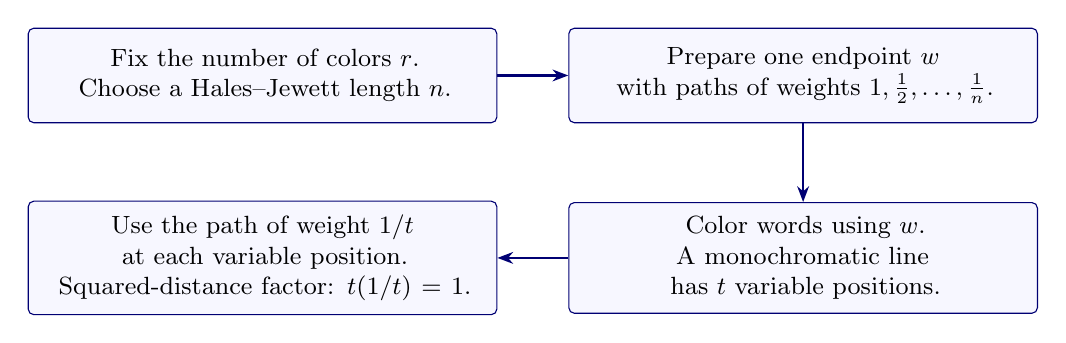
\begin{tikzpicture}[
  box/.style={draw=blue!45!black,rounded corners=2pt,fill=blue!3,
    text width=5.6cm,minimum height=1.2cm,align=center,
    inner sep=5pt,font=\small},
  flow/.style={-{Stealth[length=2mm]},thick,draw=blue!45!black}
]
\node[box] (length) {Fix the number of colors $r$.\\
  Choose a Hales--Jewett length $n$.};
\node[box,right=9mm of length] (endpoint) {Prepare one endpoint $w$\\
  with paths of weights $1,\frac12,\ldots,\frac1n$.};
\node[box,below=10mm of endpoint] (line) {Color words using $w$.\\
  A monochromatic line has $t$ variable positions.};
\node[box,left=9mm of line] (scale) {Use the path of weight $1/t$\\
  at each variable position.\\
  Squared-distance factor: $t(1/t)=1$.};
\draw[flow] (length) -- (endpoint);
\draw[flow] (endpoint) -- (line);
\draw[flow] (line) -- (scale);
\end{tikzpicture}
\caption{The order of choices in the path criterion. Every possible
variable count is accommodated before the word coloring is defined.
Choosing a path representation later leaves its endpoint unchanged;
common factors become common strings, so only the variable blocks
contribute to pairwise distances.}
\label{fig:synchronization}
\end{figure}


For each of the line's $s$ words, expand the factor
at every variable position using the chosen path ending at $w$ with
weight $1/t$. A diagonal path factor contributes one common
ultrafilter $\psi(g)$. A copy factor contributes
$p\delta_{(b_i)}p$ in role $i$: the two $p$ factors are common and
the middle factor is principal at a prescribed one-letter string.
Unexpanded fixed positions are common factors as well. The identity
of the corner group is $p$; if an empty group product occurs, it is
retained as this common factor. The expanded products therefore have
the column forms required by Lemma~\ref{paths:realization}, and all
contain the same color class $B_k$.

Apply that lemma. It produces strings $z^{(1)},\ldots,z^{(s)}$ in $B_k$. Every common
factor was realized by the same string in all roles, and every
varying factor has length one. Hence the resulting strings have equal
lengths and their entries align. Common strings contribute zero to
their pairwise squared distances. Each of the $t$ expanded paths
contributes
$\|a_i-a_j\|^2/t$ by its weight. Equation
\eqref{paths:string-distance} consequently gives
\[
\|\Phi(z^{(i)})-\Phi(z^{(j)})\|^2
=t\frac1t\|a_i-a_j\|^2
=\|a_i-a_j\|^2.
\]
Their images form a monochromatic congruent copy of $A$ in
$\mathcal E$. Lemma~\ref{paths:compactness} now supplies a finite
forcing dimension for this $r$. Since $r$ was arbitrary, $A$ is
Euclidean Ramsey.
\end{proof}

\section{From coordinate permutations to equal path endpoints}
\label{sec:groups}

We now turn the two images of Lemma~\ref{pairs:two-scale} into the
equal-endpoint paths required by Proposition~\ref{paths:criterion}.
Recall that $\mathcal E=\R^{(\N)}$, that $K$ is the free group on
the letters $\xi_z$ for $z\in\mathcal E$, and that path weights count
the squared-distance scales of their copy factors.  The two images give
paths of very different weights.  Their endpoints need not agree.
Our task is to correct those endpoints at a cost small relative to the
larger weight.

\subsection{Corrections supported on individual coordinates}

Let $M\subset K^s$ be the monoid generated by the diagonal subgroup
$\Delta K$ and the tuples $X_b=(\xi_{b_i})_{i=1}^s$ associated to
ordered congruent copies $b$ of $A$.  Thus a chosen expression for an
element of $M$ is a path using only copy factors of weight one.
Its \emph{degree} is the number of those factors; diagonal factors have
degree zero.  Degrees always refer to chosen expressions.

Suppose two paths have endpoints $D_+,D_-\in K^s$. If we can write
\[
 D_+^{-1}D_-=uv^{-1}\qquad(u,v\in M),
\]
then $D_+u=D_-v$. Appending the chosen expressions for $u$ and $v$
therefore gives equal endpoints, with added weights $\deg u$ and
$\deg v$, respectively. We will make their sum small relative to the
larger original path weight, so that correcting the endpoints retains
the small ratio of weights.

To construct these corrections, let
\[
 N=\ker\bigl(K\longrightarrow\Z,\ \xi_z\longmapsto1\bigr).
\]
For distinct labels $i,j$, write $M_{ij}$ for the image of $M$ under
projection onto coordinates $i,j$.

\begin{lemma}\label{groups:pairs}
For every $i\ne j$, the monoid $M_{ij}$ is a group containing
$N\times N$.
\end{lemma}
\begin{proof}
Put $r=\|a_i-a_j\|>0$.  Every ordered pair $z,z'\in\mathcal E$
at distance $r$ extends to an ordered congruent copy of $A$.
Indeed, send the direction of $a_j-a_i$ to $(z'-z)/r$, extend it to
an orthonormal frame for the affine span of $A$, and translate to send
$a_i$ to $z$.  The frame can be chosen inside a finite-dimensional
coordinate subspace of $\mathcal E$.

Set $x=\xi_z$ and $y=\xi_{z'}$.  Both $(x,y)$ and $(y,x)$ therefore
belong to $M_{ij}$, and
\[
 (x,y)^{-1}
   =(x^{-1},x^{-1})(y,x)(y^{-1},y^{-1})\in M_{ij}.
\]
The diagonal generators are also invertible within $M_{ij}$, so this
monoid is a group.  It contains
\[
 (x,y)(y^{-1},y^{-1})=(xy^{-1},1),
 \qquad
 (x,y)(x^{-1},x^{-1})=(1,yx^{-1}),
\]
and their conjugates by diagonal elements.

The graph on $\mathcal E$ joining points at distance $r$ is connected.
To see this, subdivide any displacement into pieces of length at most
$2r$.  The endpoints of each piece have a common point at distance $r$:
choose an appropriate perpendicular displacement from their midpoint.
An additional coordinate supplies the perpendicular direction if needed.
Differences of letters along graph edges consequently generate, after
taking their normal closure in $K$, all differences $\xi_z\xi_{z'}^{-1}$.
That normal closure is $N$, since identifying all free generators gives
the infinite cyclic group.  The two displayed types of elements and
diagonal conjugation thus give $N\times N\subset M_{ij}$.
\end{proof}

For $g\in K$, let $g^{[i]}\in K^s$ have value $g$ in coordinate $i$
and identity in every other coordinate.  Define
\[
 L_i=\{g\in K:g^{[i]}=uv^{-1}\text{ for some }u,v\in M\}.
\]
We call $uv^{-1}$ a \emph{right fraction}.  Its cost, with chosen
expressions for $u,v$, is the sum of their degrees.  For $g\in L_i$,
let $c_i(g)$ be the minimum cost of a right fraction representing
$g^{[i]}$.  The minimum exists because its possible costs form a
nonempty set of nonnegative integers.

We will only multiply right fractions when their supports permit an
explicit construction of a new denominator.  No closure assertion for
the whole set $MM^{-1}$ is needed.

\begin{lemma}\label{groups:fractions}
Each $L_i$ is a normal subgroup of $K$, and its cost satisfies
\[
 c_i(g^{-1})=c_i(g),\qquad
 c_i(kgk^{-1})=c_i(g),\qquad
 c_i(gh)\le c_i(g)+c_i(h)
\]
for $g,h\in L_i$ and $k\in K$.
Every tuple $(g_i)_{i=1}^s$ with $g_i\in L_i$ has a represented
right fraction of cost at most $\sum_i c_i(g_i)$.
Moreover,
\begin{equation}\label{groups:derived-inclusion}
 N^{(s-2)}\subset L_i\qquad(1\le i\le s),
\end{equation}
where $N^{(0)}=N$ and $N^{(r+1)}=[N^{(r)},N^{(r)}]$.
\end{lemma}
\begin{proof}
Inversion of a right fraction interchanges its numerator and denominator.
If $d=\Delta(k)$, then
\[
 (kgk^{-1})^{[i]}=(du)(dv)^{-1}
 \quad\text{whenever}\quad g^{[i]}=uv^{-1}.
\]
These operations preserve the represented cost.  Applying each operation
in both directions proves inversion and conjugation invariance.

The following multiplication rule supplies the cost estimate.  Given
any represented right fraction $uv^{-1}$ and $g\in L_i$, put
$h=v_i^{-1}gv_i$ and choose $h^{[i]}=ab^{-1}$ of cost $c_i(h)=c_i(g)$.
Then
\begin{equation}\label{groups:single-multiplication}
 uv^{-1}g^{[i]}
   =u h^{[i]}v^{-1}
   =ua b^{-1}v^{-1}
   =(ua)(vb)^{-1}.
\end{equation}
The resulting cost is at most the previous cost plus $c_i(g)$.
This proves product closure and subadditivity for $L_i$; together with
inversion and conjugation it proves normality.  Successively applying
\eqref{groups:single-multiplication} to the single-coordinate factors of
$(g_i)_i$ proves the asserted tuple cost bound.

For the derived subgroup inclusion, we also need a multiplication rule
for fractions supported on a pair of coordinates.  Suppose that
$z=cd^{-1}$ is such a fraction, supported on a pair $J$, and let
$uv^{-1}$ be any right fraction.  Since the projection of $M$ onto $J$
is a group, choose $b\in M$ such that $t=vb$ is the identity on $J$.
The tuples $t$ and $z$ commute, because their supports are disjoint.
Consequently
\begin{equation}\label{groups:pair-multiplication}
 uv^{-1}z
   =ubt^{-1}z
   =ubzt^{-1}
   =ubc d^{-1}t^{-1}
   =(ubc)(td)^{-1}.
\end{equation}
This is a right fraction of finite cost.  We require no bound on the
cost of the auxiliary $b$.

We now prove \eqref{groups:derived-inclusion} by induction on the number
of coordinates.  The proof applies to any submonoid of $K^s$ containing
the diagonal whose pair projections are groups containing $N\times N$.
For $s=2$, the whole monoid is its pair projection and contains
$N\times N$, which proves the claim.
For $s\ge3$, fix distinct indices $i,j,k$.
The monoid obtained by projecting away $j$ satisfies the same abstract
hypotheses.  By induction, every $a\in N^{(s-3)}$ has a right fraction
in that projection supported at $i$.  Lift its numerator and denominator
to $M$.  Their quotient is a right fraction $z_a$ supported on $\{i,j\}$,
with value $a$ at $i$.  Projecting away $k$ similarly gives a right
fraction $z_b$ supported on $\{i,k\}$ with any prescribed
$b\in N^{(s-3)}$ at $i$.

The four factors of $z_a z_b z_a^{-1}z_b^{-1}$ are pair-supported
right fractions; inverses remain fractions by interchanging numerator
and denominator.  Repeated use of \eqref{groups:pair-multiplication}
makes their product a right fraction.  Its only possibly nonidentity
coordinate is $i$, where its value is $[a,b]$.
Thus $[a,b]\in L_i$.  Since $L_i$ is a subgroup, it contains the subgroup
generated by all these commutators, namely $N^{(s-2)}$.
\end{proof}

Set
\begin{equation}\label{groups:cost}
 L=N^{(s-2)},\qquad c(g)=\max_{1\le i\le s}c_i(g)\quad(g\in L).
\end{equation}
The subgroup $L$ is normal in $K$.  Lemma~\ref{groups:fractions} shows
that $c$ is finite, symmetric under inversion, subadditive, and invariant
under conjugation by every element of $K$.  We have therefore identified
a subgroup of allowable endpoint corrections and a cost for each one.
We next construct long paths for which the needed corrections have
small cost relative to their degree.

\subsection{Averaging over coordinate permutations}

Let $H$ be a finite group of coordinate permutations acting on
$\mathcal E$, and let $Z\subset\mathcal E$ be a finite $H$-invariant set.
Consider represented tuples $w=(w_x)_{x\in Z}\in K^Z$ obtained by
multiplying diagonal factors and factors
\[
 (\xi_{h x})_{x\in Z},\qquad h\in H.
\]
The degree of such an expression is the number of factors of the latter
kind.  Right multiplication by a diagonal element has degree zero.
Replacing $w_x$ by $w_{h x}$ preserves the degree: it sends a generator
indexed by $g\in H$ to the generator indexed by $gh$.

\begin{lemma}\label{groups:averaging}
Let $H$ be a finite group of coordinate permutations of $\mathcal E$,
and let $Z\subset\mathcal E$ be a finite $H$-invariant set. For every
$\delta>0$, there is a tuple $w\in K^Z$ represented by diagonal
factors and factors $(\xi_{h x})_{x\in Z}$, $h\in H$, with degree
$m>0$, for which
\begin{equation}\label{groups:orbit-bound}
 w_xw_y^{-1}\in L,\qquad c(w_xw_y^{-1})\le\delta m
 \quad\text{whenever }x,y\text{ belong to the same }H\text{-orbit}.
\end{equation}
\end{lemma}
\begin{proof}
We first arrange membership in $L$, then make the costs small.
Start with $w_x=\xi_x$, represented with degree one; its differences
$w_xw_y^{-1}$ belong to $N$.

Suppose the differences on an orbit $O$ belong to $N^{(r)}$.
Choose $x_0\in O$ and right-multiply by the diagonal element
$w_{x_0}^{-1}$.  After this operation, every value on $O$ belongs to
$N^{(r)}$, and every difference on every orbit is unchanged.
Replace the resulting tuple by
\begin{equation}\label{groups:derived-average}
 w'_x=\prod_{h\in H}w_{h x},
\end{equation}
using a fixed order on $H$.  For $x\in O$, the list $(h x)_{h\in H}$
visits every point of $O$ with the same multiplicity $|H|/|O|$.
The products in \eqref{groups:derived-average} therefore have the same
image in the abelian group $N^{(r)}/N^{(r+1)}$ for every $x\in O$.
Their differences belong to $N^{(r+1)}$.

This procedure preserves any normal-subgroup condition already obtained
on another orbit.  Indeed, if $w_xw_y^{-1}\in G$ there for a normal
subgroup $G\lhd K$, corresponding factors of the two products have the
same image in $K/G$.  Their products have the same image as well.
Process the finitely many orbits, increasing the derived depth on each
to $s-2$.  Every degree stays positive, and we obtain membership in $L$
for all within-orbit differences.  When $s=2$, the initial tuple already
has this property.

Fix one orbit $O$.  Right-normalize at $x_0\in O$ once more, so all
values on $O$ lie in $L$, and write
$B=\max_{x\in O}c(w_x)$.  Put $h=|H|$.
If $h=1$, all orbits are singletons and \eqref{groups:orbit-bound}
already holds.  Hence suppose $h\ge2$.
Repeatedly perform the operation
\begin{equation}\label{groups:contract}
 w'_x=\left(\prod_{g\in H}w_{g x}\right)w_{x_0}^{-1}.
\end{equation}
For each $x\in O$, one factor in the product is $a=w_{x_0}$.
Write the product as $P a Q$.  Then
\[
 w'_x=P(aQa^{-1}),\qquad
 c(w'_x)\le c(P)+c(Q)\le(h-1)B.
\]
All new values on $O$ still lie in $L$, and their represented degree is
$h$ times the preceding degree.  Thus, after $k$ repetitions starting
from degree $m_0$, the maximum difference cost divided by degree is at
most
\begin{equation}\label{groups:contraction-rate}
 \frac{2B}{m_0}\left(\frac{h-1}{h}\right)^k.
\end{equation}
Here the factor two uses
$c(w_xw_y^{-1})\le c(w_x)+c(w_y)$.
The bound tends to zero.

It remains to check that treating this orbit does not spoil a bound on
another orbit.  If $a_jb_j^{-1}\in L$ for $1\le j\le h$, conjugation
invariance and subadditivity give
\begin{equation}\label{groups:product-bound}
 c\bigl((a_1\cdots a_h)(b_1\cdots b_h)^{-1}\bigr)
 \le\sum_{j=1}^h c(a_jb_j^{-1}).
\end{equation}
For completeness, write $A_j=a_1\cdots a_j$ and
$B_j=b_1\cdots b_j$, with $A_0=B_0=1$.  The identity
\[
 A_jB_j^{-1}
 =\bigl(A_{j-1}(a_jb_j^{-1})A_{j-1}^{-1}\bigr)
   \bigl(A_{j-1}B_{j-1}^{-1}\bigr)
\]
proves \eqref{groups:product-bound} inductively.
Consequently the product in \eqref{groups:contract} multiplies the
maximum difference cost on any other orbit by at most $h$, while
multiplying the degree by exactly $h$.  The appended common right factor
does not change differences.  Their cost divided by degree cannot
increase.  We may therefore achieve the bound $\delta$ on one orbit
after another; there are only finitely many orbits.
\end{proof}

\subsection{Equal endpoints and completion of sufficiency}

We can now compare the two paths supplied by coordinate permutations.
The preceding lemma makes their endpoint discrepancies inexpensive,
and Lemma~\ref{groups:fractions} realizes all discrepancies by actual
paths of unit-scale copies.

\begin{proposition}\label{groups:endpoints}
Suppose $q>0$ and $f_i,g_i\in\R^\ell$ satisfy
\[
 \|f_i-f_j\|^2=\|a_i-a_j\|^2,\qquad
 \|g_i-g_j\|^2=q\|a_i-a_j\|^2
 \quad(1\le i,j\le s),
\]
and each $g_i$ is a coordinate permutation of $f_i$.
For every $\delta>0$ there exist two paths with the same endpoint and
weights $\lambda>0$ and $\mu\ge0$ such that
\[
 \frac{\mu}{\lambda}\le q+s\delta.
\]
\end{proposition}
\begin{proof}
Embed $\R^\ell$ into $\mathcal E$, let $H$ be its full coordinate
permutation group, acting trivially on the remaining coordinates, and
let $Z$ be the union of the $H$-orbits of the $f_i$ and $g_i$.
It is finite, and $f_i,g_i$ lie in the same orbit for each $i$.
Apply Lemma~\ref{groups:averaging} with the given $\delta$ and let $m>0$
be the degree of its represented tuple $w$.

Restricting the same expression to the labels $f_i$ gives the endpoint
$D_+=(w_{f_i})_{i=1}^s$ of a path of weight $m$.
Restricting it to the labels $g_i$ gives the endpoint
$D_-=(w_{g_i})_{i=1}^s$ of a path of weight $qm$.
Indeed, each counted factor acts by a coordinate permutation, so it
preserves the corresponding distances; diagonal factors stay diagonal.

For each $i$, put $r_i=w_{f_i}w_{g_i}^{-1}$.  By
\eqref{groups:orbit-bound}, $r_i\in L$ and $c(r_i)\le\delta m$.
The $i$th component of $D_+^{-1}D_-$ is
\[
 w_{f_i}^{-1}w_{g_i}=w_{f_i}^{-1}r_i^{-1}w_{f_i},
\]
so it too belongs to $L$ and has cost at most $\delta m$.
Lemma~\ref{groups:fractions} supplies represented $u,v\in M$ such that
\[
 D_+^{-1}D_-=uv^{-1},\qquad
 \deg u+\deg v\le s\delta m.
\]
Thus $D_+u=D_-v$.
Writing $a=\deg u$ and $b=\deg v$, the two resulting paths have weights
\[
 \lambda=m+a>0,\qquad \mu=qm+b\ge0,
 \qquad
 \frac{\mu}{\lambda}
    \le\frac{qm+b}{m}\le q+s\delta.
\]
\end{proof}

\begin{proof}[Completion of the sufficiency implication in
Theorem~\ref{thm:classification}]
Assume the matrix condition of the theorem. By
Proposition~\ref{alg:equivalence}, the tensor condition
\eqref{alg:tensor} holds.
For every integer $n\ge1$, Lemma~\ref{pairs:two-scale} supplies two
images as in Proposition~\ref{groups:endpoints} with
$0<q<1/(2n)$.  Apply that proposition with $\delta=1/(2sn)$.
It gives equal-endpoint paths whose weight ratio is strictly less than
$1/n$.  Proposition~\ref{paths:criterion} now implies that $A$ is Ramsey.
All choices are made after fixing $n$; no bound uniform in $n$ on the
degrees or the number of coordinates is required.
\end{proof}

\section{Geometric consequences and examples}\label{cons:section}\label{sec:consequences}

The criterion separates two different questions about a spherical set:
whether its ordinary quadratic equations admit the required identity
block, and whether that solution lifts to the tensor ring. We first give
positive examples, then exhibit two failures of the lift.

\begin{corollary}\label{cons:spherical}
Every finite Euclidean Ramsey set is spherical.
\end{corollary}
\begin{proof}
A singleton is spherical. Otherwise use the notation and a matrix $P$
from Theorem~\ref{thm:classification}, and put $H=m_F(P)$, entrywise.
Multiplying the evaluation equations gives
\[
 \|a_i\|^2+\ell\cdot a_i+c=0,
 \qquad c=H_{00},\qquad
 \ell_\alpha=H_{0\alpha}+H_{\alpha0}\quad(1\le\alpha\le d).
\]
Thus all points lie on the sphere with center $-\ell/2$ and squared
radius $\|\ell\|^2/4-c$. The radius is positive because the set has
at least two distinct points. No symmetry of the constant row and
column of $H$ is needed.
\end{proof}

A finite Euclidean set is \emph{transitive} if its distance-preserving
permutations act transitively on its points.

\begin{corollary}\label{cons:transitive}
Every nonempty subset of a finite transitive Euclidean set is Ramsey.
\end{corollary}
\begin{proof}
Singletons are immediate. Let $A=\{a_1,\ldots,a_s\}\subset\R^d$,
with $s\ge2$, affinely span $\R^d$, and suppose an isometric
embedding maps $a_i$ to $y_i$ in a finite transitive set
$Y\subset\R^n$. Write $H$ for the finite group of distance-preserving
permutations of $Y$. For each $h\in H$, the map $a_i\mapsto h(y_i)$
extends to an affine isometry. Let $w_{hj}\in W=\R^{1+d}$ be its
$j$th affine coordinate row, so that $e_i(w_{hj})=(h(y_i))_j$.
The gradient Gram matrix of these $n$ rows is $I_d$.

Let $c_{hj}=((h(y_1))_j,0)\in W$, a constant affine row. The
symmetric rational tensor
\[
 T=\frac1{|H|}\sum_{h\in H}\sum_{j=1}^n
       \bigl(w_{hj}\otimes w_{hj}-c_{hj}\otimes c_{hj}\bigr)
\]
has $G(T)=I_d$. For each $i$, the multiset $(h(y_i))_{h\in H}$
contains every point of $Y$ exactly $|H|/|Y|$ times. Consequently
\[
 \sum_{h,j}(h(y_i))_j\otimes(h(y_i))_j
 =\sum_{h,j}(h(y_1))_j\otimes(h(y_1))_j,
\]
and $(e_i\otimes e_i)(T)=0$. Proposition~\ref{alg:equivalence}
and Theorem~\ref{thm:classification} now give the Ramsey property.
\end{proof}

Quadratic interpolation gives another source of tensor certificates.
The row-independence hypothesis below says that quadratic polynomials
can prescribe arbitrary values on the configuration.

\begin{proposition}\label{cons:quadratic}
Let $A=\{a_1,\ldots,a_s\}\subset\R^d$ be spherical and affinely
span $\R^d$. Put $p_i=(1,a_i)^{\mathsf T}$ and let $F$ be its
coordinate field. If the $s$ row vectors
\[
 (p_{i\alpha}p_{i\beta})_{0\le\alpha,\beta\le d}
 \quad(1\le i\le s)
\]
are linearly independent over $F$, then $A$ is Ramsey.
\end{proposition}
\begin{proof}
The singleton case is immediate, so assume $s\ge2$. Write
$N=(d+1)^2$. Sphericity gives a real matrix with spatial block
$I_d$ and quadratic values zero at every $p_i$. These requirements
are a linear system over $F$, so a solution exists over $F$ as well,
by Gaussian elimination. Denote such a matrix, written as a vector in
$F^N$, by $h$.

Let $D\in\operatorname{Mat}_{s\times N}(B)$ be the tensor evaluation
matrix, whose entry in row $i$ and column $(\alpha,\beta)$ is
$p_{i\alpha}\otimes p_{i\beta}$. Lift $h$ to $b\in B^N$ by applying
$x\mapsto x\otimes1$ entrywise. The assumed row independence allows
us to select $s$ columns of $D$ whose square submatrix $M$ has
\[
 \delta=m_F(\det M)\ne0.
\]
Let $\iota:B^s\to B^N$ insert a vector into these selected coordinates,
so that $D\iota=M$. Multiplying by $\det M$ allows us to cancel the
tensor evaluation error $Db$ through the selected columns: the adjugate
identity gives
\[
 z=(\det M)b-\iota\operatorname{adj}(M)Db\in\ker D.
\]
Since $m_F(D)h=0$, multiplication gives $m_F(z)=\delta h$.
Multiplying $z$ by $\delta^{-1}\otimes1$ therefore produces a
solution of the criterion in Theorem~\ref{thm:classification}.
This argument does not require $\det M$ to be a unit of $B$.
\end{proof}

For at most five circle points, products of two line equations supply
the required interpolation. The same observation appears in P\'alv\"olgyi's
analysis of derivation obstructions
\cite[proof of Theorem~A.2]{palvolgyi-heptagon}.

\begin{corollary}\label{cons:quadrilateral}
Every nonempty set of at most five distinct points on a circle is Ramsey.
In particular, every cyclic quadrilateral is Ramsey.
\end{corollary}
\begin{proof}
Work in the plane of the circle and extend the set, if necessary, to
five distinct points on that circle. Let $F$ be the coordinate field of
the resulting five-point set. Fix one of these points $a_i$, partition
the other four into two pairs, and take the product of affine equations for the two lines
through those pairs. No three circle points are collinear, so this
quadratic polynomial vanishes at the other four points and is nonzero
at $a_i$. Its coefficients lie in the coordinate field $F$. Rescaling
the five resulting polynomials shows that quadratic evaluation onto
$F^5$ is surjective. Its five rows are therefore independent, and
Proposition~\ref{cons:quadratic} makes the five-point set Ramsey.
A monochromatic copy of that set contains a copy of the original set.
\end{proof}

\begin{corollary}\label{cons:kites}
For every transcendental $a\in(-1,1)$, the cyclic quadrilateral
\[
 K_a=\bigl\{(-1,0),(1,0),
             (a,\sqrt{1-a^2}),(a,-\sqrt{1-a^2})\bigr\}
\]
is Ramsey and is not subtransitive.
\end{corollary}
\begin{proof}
The four points are distinct and lie on the unit circle, so
Corollary~\ref{cons:quadrilateral} makes $K_a$ Ramsey.
Leader, Russell and Walters proved that $K_a$ does not embed in any
finite transitive Euclidean set \cite[Corollary~2]{lrw-kites}.
\end{proof}

Thus the necessity direction of the Leader--Russell--Walters
subtransitive characterization fails \cite[Conjecture~A]{lrw-transitive}.
The same family also disproves their conjecture that these kites are
not Ramsey \cite[Conjecture~3]{lrw-kites}.

\subsection{Nine points on a circle}

The tensor equations can have full rank even when their multiplied
versions admit a sphere equation. The following determinant calculation
illustrates this distinction. P\'alv\"olgyi's earlier generic-seven-point
claim \cite[Theorem~A.3]{palvolgyi-heptagon} already implies its
non-Ramsey conclusion by taking a subset; the source labels its appendix
as unchecked. We give a direct proof from the tensor criterion.

\begin{proposition}\label{cons:nine}
Let $t_1,\ldots,t_9$ be algebraically independent real numbers over
$\Q$. The nine points
\[
 a_i=\left(\frac{1-t_i^2}{1+t_i^2},
                \frac{2t_i}{1+t_i^2}\right),\qquad 1\le i\le9,
\]
form a spherical set that is not Ramsey.
\end{proposition}
\begin{proof}
The parametrization lies on the unit circle and is injective, since
$t_i=(a_i)_2/(1+(a_i)_1)$. Thus the points are distinct, affinely span
$\R^2$, and have coordinate field $F=\Q(t_1,\ldots,t_9)$.
Algebraic independence identifies this field with a rational function
field. Consequently $B=F\otimes_\Q F$ is the localization of
$\Q[T_1,\ldots,T_9,U_1,\ldots,U_9]$ obtained by inverting all
nonzero polynomials in the $T$ variables alone and all nonzero
polynomials in the $U$ variables alone. In particular, $B$ is a domain
and embeds in $\Q(T_1,\ldots,T_9,U_1,\ldots,U_9)$.

Put
\[
 p(t)=\left(1,\frac{1-t^2}{1+t^2},\frac{2t}{1+t^2}\right)^{\mathsf T}.
\]
Over this fraction field, the nine tensor evaluation equations have
coefficient matrix $D$ with rows
$(p_\alpha(T_i)p_\beta(U_i))_{0\le\alpha,\beta\le2}$.
We claim that $\det D\ne0$. To check the claim, specialize the nine
pairs $(T_i,U_i)$ to the grid $\{0,1,-1\}^2$, with both coordinates
ordered as $0,1,-1$.
All denominators in the displayed matrix remain nonzero. The resulting
matrix is the ordinary Kronecker product $C\otimes C$, where
\[
 C=\begin{pmatrix}1&1&0\\1&0&1\\1&0&-1\end{pmatrix},
 \qquad \det C=2.
\]
Its determinant is $2^6=64$, proving the claim. This evaluates the
specific determinant expression; no specialization of the entire
localized ring $B$ is asserted.

Thus the only solution of $D\,\operatorname{vec}(P)=0$ over the
fraction field is $P=0$. Injectivity of the embedding of $B$ shows
that the same holds over $B$. Such a matrix cannot have multiplied
spatial block $I_2$, so Theorem~\ref{thm:classification} excludes the
Ramsey property.
\end{proof}

\subsection{Three concentric squares}

A second example uses only one transcendental parameter. It also shows
how a derivation can detect the failure of the tensor equations directly
inside the coordinate field. Its weighted cancellation is related to
the derivation obstruction in P\'alv\"olgyi's smaller circular example
\cite[Theorem~1]{palvolgyi-heptagon}; the calculation below is independent
of that proof. The parameter is Liouville's constant
\cite{liouville1851}.

\begin{proposition}\label{cons:twelve}
Set
\[
 t=\sum_{m=1}^{\infty}10^{-m!},\qquad
 u=\frac{1-t^2}{1+t^2},\qquad v=\frac{2t}{1+t^2},
 \qquad Q_0=\{(\pm1,0),(0,\pm1)\},
\]
and define
\[
 R_+=\begin{pmatrix}u&-v\\v&u\end{pmatrix},\qquad
 R_-=\begin{pmatrix}u&v\\-v&u\end{pmatrix},\qquad
 X=R_+Q_0\cup R_-Q_0\cup Q_0.
\]
Then $X$ is a twelve-point subset of the unit circle that is not Ramsey.
\end{proposition}
\begin{proof}
First, $0.11<t<0.12$ and $t$ is transcendental. Indeed, the rational
partial sums $t_m=p_m/q_m$, with $q_m=10^{m!}$, satisfy
\[
 0<t-t_m<2q_m^{-(m+1)}\qquad(m\ge2).
\]
If $t$ had an irreducible polynomial $P\in\Z[T]$ of degree $d$, then
$P(t_m)\ne0$ and $|P(t_m)|\ge q_m^{-d}$. A bound $C\ge1$ for
$|P'|$ on $[0,1]$ would give
$q_m^{-d}<2Cq_m^{-(m+1)}$, a contradiction for large $m$.
The rotations $R_+$ and $R_-$ have angles $\theta=2\arctan t$ and
$-\theta$, where $0<\theta<\pi/4$. Their differences from each other
and from zero are nonzero and smaller than $\pi/2$ in absolute value.
Hence the three squares are disjoint. They lie on the unit circle,
and $Q_0$ already affinely spans the plane.

The coordinate field of $X$ is $F=\Q(t)$: its coordinates include
$u,v$, and $t=v/(1+u)$. On this field define the derivation
\[
 \partial=\frac{1+t^2}{2}\frac{d}{dt}.
\]
It satisfies $\partial u=-v$ and $\partial v=u$.
Write $R_0=I_2$, label the points by $x_{\epsilon,q}=R_\epsilon q$
for $\epsilon\in\{+,-,0\}$ and $q\in Q_0$, and assign weights
$\beta_{+,q}=\beta_{-,q}=1$, $\beta_{0,q}=-2$.
For these twelve labels put $p_i=(1,x_i)^{\mathsf T}$.
We have the three augmented moment identities
\begin{equation}\label{cons:derivation-moments}
 \sum_i\beta_i p_ip_i^{\mathsf T}=0,\qquad
 \sum_i\beta_i(\partial p_i)p_i^{\mathsf T}=0,\qquad
 \sum_i\beta_i(\partial p_i)(\partial p_i)^{\mathsf T}
       =\begin{pmatrix}0&0\\0&4I_2\end{pmatrix}.
\end{equation}
Here the block sizes are $1$ and $2$. To verify them, use
$\sum_{q\in Q_0}q=0$ and $\sum_{q\in Q_0}qq^{\mathsf T}=2I_2$.
With $J=\left(\begin{smallmatrix}0&-1\\1&0\end{smallmatrix}\right)$,
the derivatives are
$\partial R_+=R_+J$, $\partial R_-=-R_-J$, and
$\partial R_0=0$. The first spatial moment is
$2(1+1-2)I_2=0$; the mixed moment is $2J-2J=0$;
and the derivative moment is $2I_2+2I_2=4I_2$.
The constant and vector entries vanish by the same square symmetries.

Define the $\Q$-linear map $\Phi:F\otimes_\Q F\to F$ by
$\Phi(a\otimes b)=(\partial a)(\partial b)$.
For every $P\in\operatorname{Mat}_3(B)$, the product rule and
\eqref{cons:derivation-moments} give
\begin{equation}\label{cons:derivation-obstruction}
 \sum_i\beta_i\Phi\bigl((p_i\otimes1)^{\mathsf T}
                         P(1\otimes p_i)\bigr)
       =4\sum_{\alpha=1}^2 m_F(P_{\alpha\alpha}).
\end{equation}
For completeness, expand each entry of $P$ into pure tensors
$a\otimes b$. In
$\partial(p_{i\alpha}a)\partial(p_{i\beta}b)$, the terms involving
$\partial a$ or $\partial b$ vanish after summing with $\beta_i$ by
the first two moment identities and the transpose of the second.
The remaining term is $ab(\partial p_{i\alpha})
(\partial p_{i\beta})$, and the third identity gives exactly the
right side of \eqref{cons:derivation-obstruction}.

A matrix satisfying the classification criterion would make the
left side zero and the right side $8$. This contradiction proves the
claim. The argument uses a derivation only on $F$, and imposes no
regularity condition on the colorings in the Ramsey definition.
\end{proof}

\bibliographystyle{plain}
\bibliography{refs}
\end{document}
